\section{Application's design}
QuizFight's information model is depicted in Figure~\ref{fig:quizfighter}. The main entry point is \texttt{SignInActivity}. Our game, in its very first version, requires the user to sign in with Google Games. Hence, \texttt{SignInActivity} simply shows a button allowing the sign in. The user's dashboard is \texttt{HomeActivity}. Here the player can see their previous duels, both the completed and the pending ones. By tapping on a duel, a complete report of the result is shown. When the duel has not been completed and when a new round is actually available (i.e. when both the player and their opponent completed the previous round), a button asking the user for answering the next questions is shown. Since showing every duel would incur in a bad user experience we show only a limited number. We then provide a way to see the complete lists.
\begin{figure}[t]
	\centering
	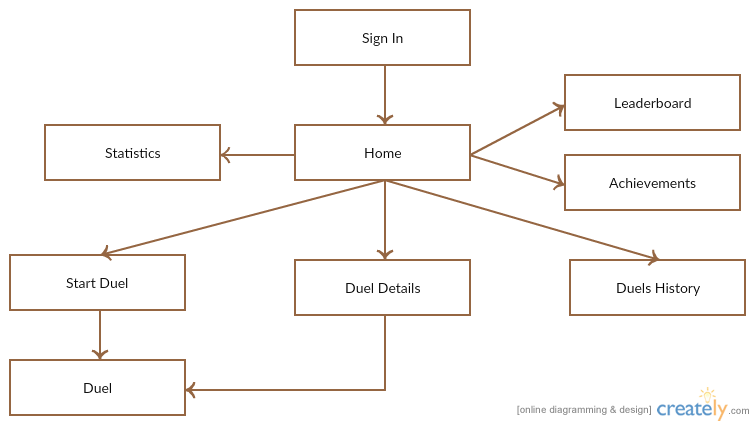
\includegraphics[width=0.9\linewidth]{QuizFightER}
	\caption{QuizFight's information model}
	\label{fig:quizfighter}
\end{figure}

From \texttt{HomeActivity} a user can also see their current situation in terms of ranks and achievements. That information is directly retrieved and shown using Google's services. In addition, QuizFight offers the possibility to take a look at a user's statistics, such as the number of duels (or rounds) won versus the number of duels (or rounds) played and the correct answers. Finally, there is the possibility to sign in with Facebook, for daring the user's friends.

By tapping on the fight button it is possible to start a new duel. Here, QuizFight currently provides three player choice modes: 
\begin{itemize}
	\item \textbf{random};
	\item selected from the \textbf{leaderboard};
	\item selected from the \textbf{Facebook's friends list}.
\end{itemize}

After that \texttt{DuelActivity} is shown and the user is able to answer the round's questions. At every answer a visual feedback is given. As usual, if the answer was correct it is highlighted in green; otherwise the wrong answer is highlighted in red and the correct one in green. At the round's ending a dialog is shown for notifying the user about their actual round's score. If both the player and the opponent have terminated the current round they are both notified about a new round available (if any), or about the duel's ending (with the final score). 